\documentclass[twoside]{book}

% Packages required by doxygen
\usepackage{fixltx2e}
\usepackage{calc}
\usepackage{doxygen}
\usepackage[export]{adjustbox} % also loads graphicx
\usepackage{graphicx}
\usepackage[utf8]{inputenc}
\usepackage{makeidx}
\usepackage{multicol}
\usepackage{multirow}
\PassOptionsToPackage{warn}{textcomp}
\usepackage{textcomp}
\usepackage[nointegrals]{wasysym}
\usepackage[table]{xcolor}

% Font selection
\usepackage[T1]{fontenc}
\usepackage[scaled=.90]{helvet}
\usepackage{courier}
\usepackage{amssymb}
\usepackage{sectsty}
\renewcommand{\familydefault}{\sfdefault}
\allsectionsfont{%
  \fontseries{bc}\selectfont%
  \color{darkgray}%
}
\renewcommand{\DoxyLabelFont}{%
  \fontseries{bc}\selectfont%
  \color{darkgray}%
}
\newcommand{\+}{\discretionary{\mbox{\scriptsize$\hookleftarrow$}}{}{}}

% Page & text layout
\usepackage{geometry}
\geometry{%
  a4paper,%
  top=2.5cm,%
  bottom=2.5cm,%
  left=2.5cm,%
  right=2.5cm%
}
\tolerance=750
\hfuzz=15pt
\hbadness=750
\setlength{\emergencystretch}{15pt}
\setlength{\parindent}{0cm}
\setlength{\parskip}{3ex plus 2ex minus 2ex}
\makeatletter
\renewcommand{\paragraph}{%
  \@startsection{paragraph}{4}{0ex}{-1.0ex}{1.0ex}{%
    \normalfont\normalsize\bfseries\SS@parafont%
  }%
}
\renewcommand{\subparagraph}{%
  \@startsection{subparagraph}{5}{0ex}{-1.0ex}{1.0ex}{%
    \normalfont\normalsize\bfseries\SS@subparafont%
  }%
}
\makeatother

% Headers & footers
\usepackage{fancyhdr}
\pagestyle{fancyplain}
\fancyhead[LE]{\fancyplain{}{\bfseries\thepage}}
\fancyhead[CE]{\fancyplain{}{}}
\fancyhead[RE]{\fancyplain{}{\bfseries\leftmark}}
\fancyhead[LO]{\fancyplain{}{\bfseries\rightmark}}
\fancyhead[CO]{\fancyplain{}{}}
\fancyhead[RO]{\fancyplain{}{\bfseries\thepage}}
\fancyfoot[LE]{\fancyplain{}{}}
\fancyfoot[CE]{\fancyplain{}{}}
\fancyfoot[RE]{\fancyplain{}{\bfseries\scriptsize Generated by Doxygen }}
\fancyfoot[LO]{\fancyplain{}{\bfseries\scriptsize Generated by Doxygen }}
\fancyfoot[CO]{\fancyplain{}{}}
\fancyfoot[RO]{\fancyplain{}{}}
\renewcommand{\footrulewidth}{0.4pt}
\renewcommand{\chaptermark}[1]{%
  \markboth{#1}{}%
}
\renewcommand{\sectionmark}[1]{%
  \markright{\thesection\ #1}%
}

% Indices & bibliography
\usepackage{natbib}
\usepackage[titles]{tocloft}
\setcounter{tocdepth}{3}
\setcounter{secnumdepth}{5}
\makeindex

% Hyperlinks (required, but should be loaded last)
\usepackage{ifpdf}
\ifpdf
  \usepackage[pdftex,pagebackref=true]{hyperref}
\else
  \usepackage[ps2pdf,pagebackref=true]{hyperref}
\fi
\hypersetup{%
  colorlinks=true,%
  linkcolor=blue,%
  citecolor=blue,%
  unicode%
}

% Custom commands
\newcommand{\clearemptydoublepage}{%
  \newpage{\pagestyle{empty}\cleardoublepage}%
}

\usepackage{caption}
\captionsetup{labelsep=space,justification=centering,font={bf},singlelinecheck=off,skip=4pt,position=top}

%===== C O N T E N T S =====

\begin{document}

% Titlepage & ToC
\hypersetup{pageanchor=false,
             bookmarksnumbered=true,
             pdfencoding=unicode
            }
\pagenumbering{roman}
\begin{titlepage}
\vspace*{7cm}
\begin{center}%
{\Large My Project }\\
\vspace*{1cm}
{\large Generated by Doxygen 1.8.11}\\
\end{center}
\end{titlepage}
\clearemptydoublepage
\tableofcontents
\clearemptydoublepage
\pagenumbering{arabic}
\hypersetup{pageanchor=true}

%--- Begin generated contents ---
\chapter{Class Index}
\section{Class List}
Here are the classes, structs, unions and interfaces with brief descriptions\+:\begin{DoxyCompactList}
\item\contentsline{section}{\hyperlink{structnode}{node} }{\pageref{structnode}}{}
\item\contentsline{section}{\hyperlink{structnode1}{node1} }{\pageref{structnode1}}{}
\item\contentsline{section}{\hyperlink{structnode__info}{node\+\_\+info} }{\pageref{structnode__info}}{}
\end{DoxyCompactList}

\chapter{File Index}
\section{File List}
Here is a list of all files with brief descriptions\+:\begin{DoxyCompactList}
\item\contentsline{section}{\hyperlink{Lab1_8c}{Lab1.\+c} }{\pageref{Lab1_8c}}{}
\end{DoxyCompactList}

\chapter{Class Documentation}
\hypertarget{classFlyweightCharacter}{}\section{Flyweight\+Character Class Reference}
\label{classFlyweightCharacter}\index{Flyweight\+Character@{Flyweight\+Character}}
\subsection*{Public Member Functions}
\begin{DoxyCompactItemize}
\item 
\hyperlink{classFlyweightCharacter_a6d2fea212508e56523ab4d4d7ad583d4}{Flyweight\+Character} (unsigned short \hyperlink{classFlyweightCharacter_ad2633bab3a73c5fac2b3d251bf5c2bfe}{font\+Size\+Index}, unsigned short \hyperlink{classFlyweightCharacter_ab528a214bcb91ccc0016fd0cbae331af}{font\+Name\+Index}, unsigned short \hyperlink{classFlyweightCharacter_a55c3d15287653717920c8b498d904a08}{position\+In\+Stream})
\item 
void \hyperlink{classFlyweightCharacter_abd3d3cf3508cf18403546e835280ca50}{print} ()
\item 
\hyperlink{classFlyweightCharacter_af7272d0e63182f2bd32032d09d38198d}{$\sim$\+Flyweight\+Character} ()
\end{DoxyCompactItemize}
\subsection*{Private Attributes}
\begin{DoxyCompactItemize}
\item 
unsigned short \hyperlink{classFlyweightCharacter_ad2633bab3a73c5fac2b3d251bf5c2bfe}{font\+Size\+Index}
\item 
unsigned short \hyperlink{classFlyweightCharacter_ab528a214bcb91ccc0016fd0cbae331af}{font\+Name\+Index}
\item 
unsigned \hyperlink{classFlyweightCharacter_a55c3d15287653717920c8b498d904a08}{position\+In\+Stream}
\end{DoxyCompactItemize}


\subsection{Constructor \& Destructor Documentation}
\index{Flyweight\+Character@{Flyweight\+Character}!Flyweight\+Character@{Flyweight\+Character}}
\index{Flyweight\+Character@{Flyweight\+Character}!Flyweight\+Character@{Flyweight\+Character}}
\subsubsection[{\texorpdfstring{Flyweight\+Character(unsigned short font\+Size\+Index, unsigned short font\+Name\+Index, unsigned short position\+In\+Stream)}{FlyweightCharacter(unsigned short fontSizeIndex, unsigned short fontNameIndex, unsigned short positionInStream)}}]{\setlength{\rightskip}{0pt plus 5cm}Flyweight\+Character\+::\+Flyweight\+Character (
\begin{DoxyParamCaption}
\item[{unsigned short}]{font\+Size\+Index, }
\item[{unsigned short}]{font\+Name\+Index, }
\item[{unsigned short}]{position\+In\+Stream}
\end{DoxyParamCaption}
)\hspace{0.3cm}{\ttfamily [inline]}}\hypertarget{classFlyweightCharacter_a6d2fea212508e56523ab4d4d7ad583d4}{}\label{classFlyweightCharacter_a6d2fea212508e56523ab4d4d7ad583d4}

\begin{DoxyCode}
48                                                                                                            
              :
49         \hyperlink{classFlyweightCharacter_ad2633bab3a73c5fac2b3d251bf5c2bfe}{fontSizeIndex}(\hyperlink{classFlyweightCharacter_ad2633bab3a73c5fac2b3d251bf5c2bfe}{fontSizeIndex}), \hyperlink{classFlyweightCharacter_ab528a214bcb91ccc0016fd0cbae331af}{fontNameIndex}(
      \hyperlink{classFlyweightCharacter_ab528a214bcb91ccc0016fd0cbae331af}{fontNameIndex}), \hyperlink{classFlyweightCharacter_a55c3d15287653717920c8b498d904a08}{positionInStream}(\hyperlink{classFlyweightCharacter_a55c3d15287653717920c8b498d904a08}{positionInStream}) \{\}
\end{DoxyCode}
\index{Flyweight\+Character@{Flyweight\+Character}!````~Flyweight\+Character@{$\sim$\+Flyweight\+Character}}
\index{````~Flyweight\+Character@{$\sim$\+Flyweight\+Character}!Flyweight\+Character@{Flyweight\+Character}}
\subsubsection[{\texorpdfstring{$\sim$\+Flyweight\+Character()}{~FlyweightCharacter()}}]{\setlength{\rightskip}{0pt plus 5cm}Flyweight\+Character\+::$\sim$\+Flyweight\+Character (
\begin{DoxyParamCaption}
{}
\end{DoxyParamCaption}
)\hspace{0.3cm}{\ttfamily [inline]}}\hypertarget{classFlyweightCharacter_af7272d0e63182f2bd32032d09d38198d}{}\label{classFlyweightCharacter_af7272d0e63182f2bd32032d09d38198d}

\begin{DoxyCode}
55 \{\}
\end{DoxyCode}


\subsection{Member Function Documentation}
\index{Flyweight\+Character@{Flyweight\+Character}!print@{print}}
\index{print@{print}!Flyweight\+Character@{Flyweight\+Character}}
\subsubsection[{\texorpdfstring{print()}{print()}}]{\setlength{\rightskip}{0pt plus 5cm}void Flyweight\+Character\+::print (
\begin{DoxyParamCaption}
{}
\end{DoxyParamCaption}
)\hspace{0.3cm}{\ttfamily [inline]}}\hypertarget{classFlyweightCharacter_abd3d3cf3508cf18403546e835280ca50}{}\label{classFlyweightCharacter_abd3d3cf3508cf18403546e835280ca50}

\begin{DoxyCode}
50                  \{
51         std::cout << \textcolor{stringliteral}{"Font Size: "} << 
      \hyperlink{classFlyweightCharacterAbstractBuilder_ad218358c55dae716e3ac08f453e5ab0a}{FlyweightCharacterAbstractBuilder::fontSizes}[
      \hyperlink{classFlyweightCharacter_ad2633bab3a73c5fac2b3d251bf5c2bfe}{fontSizeIndex}]
52             << \textcolor{stringliteral}{", font Name: "} << \hyperlink{classFlyweightCharacterAbstractBuilder_a9b25dfdcb7fb87b00acb05616ba50dc2}{FlyweightCharacterAbstractBuilder::fontNames}
      [\hyperlink{classFlyweightCharacter_ab528a214bcb91ccc0016fd0cbae331af}{fontNameIndex}]
53             << \textcolor{stringliteral}{", character stream position: "} << \hyperlink{classFlyweightCharacter_a55c3d15287653717920c8b498d904a08}{positionInStream} << std::endl;
54     \}
\end{DoxyCode}


\subsection{Member Data Documentation}
\index{Flyweight\+Character@{Flyweight\+Character}!font\+Name\+Index@{font\+Name\+Index}}
\index{font\+Name\+Index@{font\+Name\+Index}!Flyweight\+Character@{Flyweight\+Character}}
\subsubsection[{\texorpdfstring{font\+Name\+Index}{fontNameIndex}}]{\setlength{\rightskip}{0pt plus 5cm}unsigned short Flyweight\+Character\+::font\+Name\+Index\hspace{0.3cm}{\ttfamily [private]}}\hypertarget{classFlyweightCharacter_ab528a214bcb91ccc0016fd0cbae331af}{}\label{classFlyweightCharacter_ab528a214bcb91ccc0016fd0cbae331af}
\index{Flyweight\+Character@{Flyweight\+Character}!font\+Size\+Index@{font\+Size\+Index}}
\index{font\+Size\+Index@{font\+Size\+Index}!Flyweight\+Character@{Flyweight\+Character}}
\subsubsection[{\texorpdfstring{font\+Size\+Index}{fontSizeIndex}}]{\setlength{\rightskip}{0pt plus 5cm}unsigned short Flyweight\+Character\+::font\+Size\+Index\hspace{0.3cm}{\ttfamily [private]}}\hypertarget{classFlyweightCharacter_ad2633bab3a73c5fac2b3d251bf5c2bfe}{}\label{classFlyweightCharacter_ad2633bab3a73c5fac2b3d251bf5c2bfe}
\index{Flyweight\+Character@{Flyweight\+Character}!position\+In\+Stream@{position\+In\+Stream}}
\index{position\+In\+Stream@{position\+In\+Stream}!Flyweight\+Character@{Flyweight\+Character}}
\subsubsection[{\texorpdfstring{position\+In\+Stream}{positionInStream}}]{\setlength{\rightskip}{0pt plus 5cm}unsigned Flyweight\+Character\+::position\+In\+Stream\hspace{0.3cm}{\ttfamily [private]}}\hypertarget{classFlyweightCharacter_a55c3d15287653717920c8b498d904a08}{}\label{classFlyweightCharacter_a55c3d15287653717920c8b498d904a08}


The documentation for this class was generated from the following file\+:\begin{DoxyCompactItemize}
\item 
\hyperlink{Flyweight_8cpp}{Flyweight.\+cpp}\end{DoxyCompactItemize}

\hypertarget{classFlyweightCharacterAbstractBuilder}{}\section{Flyweight\+Character\+Abstract\+Builder Class Reference}
\label{classFlyweightCharacterAbstractBuilder}\index{Flyweight\+Character\+Abstract\+Builder@{Flyweight\+Character\+Abstract\+Builder}}
\subsection*{Static Public Member Functions}
\begin{DoxyCompactItemize}
\item 
static void \hyperlink{classFlyweightCharacterAbstractBuilder_ac5913cdc99a7af95a502d2665106a21f}{set\+Fonts\+And\+Names} ()
\item 
static \hyperlink{classFlyweightCharacter}{Flyweight\+Character} \hyperlink{classFlyweightCharacterAbstractBuilder_a06267194fa4fda26efc159c0e3b69762}{create\+Flyweight\+Character} (unsigned short font\+Size\+Index, unsigned short font\+Name\+Index, unsigned short position\+In\+Stream)
\end{DoxyCompactItemize}
\subsection*{Static Public Attributes}
\begin{DoxyCompactItemize}
\item 
static std\+::vector$<$ float $>$ \hyperlink{classFlyweightCharacterAbstractBuilder_ad218358c55dae716e3ac08f453e5ab0a}{font\+Sizes}
\item 
static std\+::vector$<$ std\+::string $>$ \hyperlink{classFlyweightCharacterAbstractBuilder_a9b25dfdcb7fb87b00acb05616ba50dc2}{font\+Names}
\end{DoxyCompactItemize}
\subsection*{Private Member Functions}
\begin{DoxyCompactItemize}
\item 
\hyperlink{classFlyweightCharacterAbstractBuilder_a32d31a8c1a4d7987fef5273d86ec3f7c}{Flyweight\+Character\+Abstract\+Builder} ()
\item 
\hyperlink{classFlyweightCharacterAbstractBuilder_a0553f2afdf91ca5e4b7821c1e3895595}{$\sim$\+Flyweight\+Character\+Abstract\+Builder} ()
\end{DoxyCompactItemize}


\subsection{Constructor \& Destructor Documentation}
\index{Flyweight\+Character\+Abstract\+Builder@{Flyweight\+Character\+Abstract\+Builder}!Flyweight\+Character\+Abstract\+Builder@{Flyweight\+Character\+Abstract\+Builder}}
\index{Flyweight\+Character\+Abstract\+Builder@{Flyweight\+Character\+Abstract\+Builder}!Flyweight\+Character\+Abstract\+Builder@{Flyweight\+Character\+Abstract\+Builder}}
\subsubsection[{\texorpdfstring{Flyweight\+Character\+Abstract\+Builder()}{FlyweightCharacterAbstractBuilder()}}]{\setlength{\rightskip}{0pt plus 5cm}Flyweight\+Character\+Abstract\+Builder\+::\+Flyweight\+Character\+Abstract\+Builder (
\begin{DoxyParamCaption}
{}
\end{DoxyParamCaption}
)\hspace{0.3cm}{\ttfamily [inline]}, {\ttfamily [private]}}\hypertarget{classFlyweightCharacterAbstractBuilder_a32d31a8c1a4d7987fef5273d86ec3f7c}{}\label{classFlyweightCharacterAbstractBuilder_a32d31a8c1a4d7987fef5273d86ec3f7c}

\begin{DoxyCode}
16 \{\}
\end{DoxyCode}
\index{Flyweight\+Character\+Abstract\+Builder@{Flyweight\+Character\+Abstract\+Builder}!````~Flyweight\+Character\+Abstract\+Builder@{$\sim$\+Flyweight\+Character\+Abstract\+Builder}}
\index{````~Flyweight\+Character\+Abstract\+Builder@{$\sim$\+Flyweight\+Character\+Abstract\+Builder}!Flyweight\+Character\+Abstract\+Builder@{Flyweight\+Character\+Abstract\+Builder}}
\subsubsection[{\texorpdfstring{$\sim$\+Flyweight\+Character\+Abstract\+Builder()}{~FlyweightCharacterAbstractBuilder()}}]{\setlength{\rightskip}{0pt plus 5cm}Flyweight\+Character\+Abstract\+Builder\+::$\sim$\+Flyweight\+Character\+Abstract\+Builder (
\begin{DoxyParamCaption}
{}
\end{DoxyParamCaption}
)\hspace{0.3cm}{\ttfamily [inline]}, {\ttfamily [private]}}\hypertarget{classFlyweightCharacterAbstractBuilder_a0553f2afdf91ca5e4b7821c1e3895595}{}\label{classFlyweightCharacterAbstractBuilder_a0553f2afdf91ca5e4b7821c1e3895595}

\begin{DoxyCode}
17 \{\}
\end{DoxyCode}


\subsection{Member Function Documentation}
\index{Flyweight\+Character\+Abstract\+Builder@{Flyweight\+Character\+Abstract\+Builder}!create\+Flyweight\+Character@{create\+Flyweight\+Character}}
\index{create\+Flyweight\+Character@{create\+Flyweight\+Character}!Flyweight\+Character\+Abstract\+Builder@{Flyweight\+Character\+Abstract\+Builder}}
\subsubsection[{\texorpdfstring{create\+Flyweight\+Character(unsigned short font\+Size\+Index, unsigned short font\+Name\+Index, unsigned short position\+In\+Stream)}{createFlyweightCharacter(unsigned short fontSizeIndex, unsigned short fontNameIndex, unsigned short positionInStream)}}]{\setlength{\rightskip}{0pt plus 5cm}{\bf Flyweight\+Character} Flyweight\+Character\+Abstract\+Builder\+::create\+Flyweight\+Character (
\begin{DoxyParamCaption}
\item[{unsigned short}]{font\+Size\+Index, }
\item[{unsigned short}]{font\+Name\+Index, }
\item[{unsigned short}]{position\+In\+Stream}
\end{DoxyParamCaption}
)\hspace{0.3cm}{\ttfamily [static]}}\hypertarget{classFlyweightCharacterAbstractBuilder_a06267194fa4fda26efc159c0e3b69762}{}\label{classFlyweightCharacterAbstractBuilder_a06267194fa4fda26efc159c0e3b69762}

\begin{DoxyCode}
58                                                                                                            
                                                                     \{
59     \hyperlink{classFlyweightCharacter}{FlyweightCharacter} fc(fontSizeIndex, fontNameIndex, positionInStream);
60 
61     \textcolor{keywordflow}{return} fc;
62 \}
\end{DoxyCode}
\index{Flyweight\+Character\+Abstract\+Builder@{Flyweight\+Character\+Abstract\+Builder}!set\+Fonts\+And\+Names@{set\+Fonts\+And\+Names}}
\index{set\+Fonts\+And\+Names@{set\+Fonts\+And\+Names}!Flyweight\+Character\+Abstract\+Builder@{Flyweight\+Character\+Abstract\+Builder}}
\subsubsection[{\texorpdfstring{set\+Fonts\+And\+Names()}{setFontsAndNames()}}]{\setlength{\rightskip}{0pt plus 5cm}void Flyweight\+Character\+Abstract\+Builder\+::set\+Fonts\+And\+Names (
\begin{DoxyParamCaption}
{}
\end{DoxyParamCaption}
)\hspace{0.3cm}{\ttfamily [static]}}\hypertarget{classFlyweightCharacterAbstractBuilder_ac5913cdc99a7af95a502d2665106a21f}{}\label{classFlyweightCharacterAbstractBuilder_ac5913cdc99a7af95a502d2665106a21f}

\begin{DoxyCode}
30                                                          \{
31     \hyperlink{classFlyweightCharacterAbstractBuilder_ad218358c55dae716e3ac08f453e5ab0a}{fontSizes}[0] = 1.0;
32     \hyperlink{classFlyweightCharacterAbstractBuilder_ad218358c55dae716e3ac08f453e5ab0a}{fontSizes}[1] = 1.5;
33     \hyperlink{classFlyweightCharacterAbstractBuilder_ad218358c55dae716e3ac08f453e5ab0a}{fontSizes}[2] = 2.0;
34 
35     \hyperlink{classFlyweightCharacterAbstractBuilder_a9b25dfdcb7fb87b00acb05616ba50dc2}{fontNames}[0] = \textcolor{stringliteral}{"first\_font"};
36     \hyperlink{classFlyweightCharacterAbstractBuilder_a9b25dfdcb7fb87b00acb05616ba50dc2}{fontNames}[1] = \textcolor{stringliteral}{"second\_font"};
37     \hyperlink{classFlyweightCharacterAbstractBuilder_a9b25dfdcb7fb87b00acb05616ba50dc2}{fontNames}[2] = \textcolor{stringliteral}{"third\_font"};
38 \}
\end{DoxyCode}


\subsection{Member Data Documentation}
\index{Flyweight\+Character\+Abstract\+Builder@{Flyweight\+Character\+Abstract\+Builder}!font\+Names@{font\+Names}}
\index{font\+Names@{font\+Names}!Flyweight\+Character\+Abstract\+Builder@{Flyweight\+Character\+Abstract\+Builder}}
\subsubsection[{\texorpdfstring{font\+Names}{fontNames}}]{\setlength{\rightskip}{0pt plus 5cm}std\+::vector$<$ std\+::string $>$ Flyweight\+Character\+Abstract\+Builder\+::font\+Names\hspace{0.3cm}{\ttfamily [static]}}\hypertarget{classFlyweightCharacterAbstractBuilder_a9b25dfdcb7fb87b00acb05616ba50dc2}{}\label{classFlyweightCharacterAbstractBuilder_a9b25dfdcb7fb87b00acb05616ba50dc2}
\index{Flyweight\+Character\+Abstract\+Builder@{Flyweight\+Character\+Abstract\+Builder}!font\+Sizes@{font\+Sizes}}
\index{font\+Sizes@{font\+Sizes}!Flyweight\+Character\+Abstract\+Builder@{Flyweight\+Character\+Abstract\+Builder}}
\subsubsection[{\texorpdfstring{font\+Sizes}{fontSizes}}]{\setlength{\rightskip}{0pt plus 5cm}std\+::vector$<$ float $>$ Flyweight\+Character\+Abstract\+Builder\+::font\+Sizes\hspace{0.3cm}{\ttfamily [static]}}\hypertarget{classFlyweightCharacterAbstractBuilder_ad218358c55dae716e3ac08f453e5ab0a}{}\label{classFlyweightCharacterAbstractBuilder_ad218358c55dae716e3ac08f453e5ab0a}


The documentation for this class was generated from the following file\+:\begin{DoxyCompactItemize}
\item 
\hyperlink{Flyweight_8cpp}{Flyweight.\+cpp}\end{DoxyCompactItemize}

\chapter{File Documentation}
\hypertarget{Flyweight_8cpp}{}\section{Flyweight.\+cpp File Reference}
\label{Flyweight_8cpp}\index{Flyweight.\+cpp@{Flyweight.\+cpp}}
{\ttfamily \#include $<$iostream$>$}\\*
{\ttfamily \#include $<$string$>$}\\*
{\ttfamily \#include $<$vector$>$}\\*
Include dependency graph for Flyweight.\+cpp\+:
\nopagebreak
\begin{figure}[H]
\begin{center}
\leavevmode
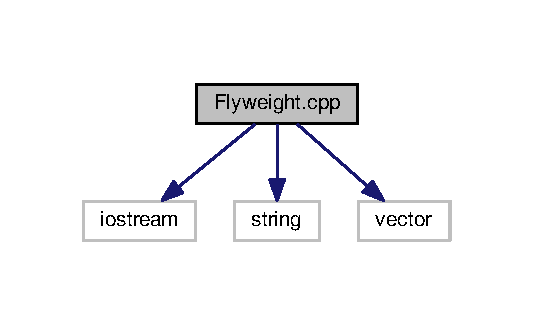
\includegraphics[width=256pt]{Flyweight_8cpp__incl}
\end{center}
\end{figure}
\subsection*{Classes}
\begin{DoxyCompactItemize}
\item 
class \hyperlink{classFlyweightCharacterAbstractBuilder}{Flyweight\+Character\+Abstract\+Builder}
\item 
class \hyperlink{classFlyweightCharacter}{Flyweight\+Character}
\end{DoxyCompactItemize}
\subsection*{Macros}
\begin{DoxyCompactItemize}
\item 
\#define \hyperlink{Flyweight_8cpp_a3d4f434225794ef00f375fcde5fc00cf}{N\+U\+M\+B\+E\+R\+\_\+\+O\+F\+\_\+\+S\+A\+M\+E\+\_\+\+T\+Y\+P\+E\+\_\+\+C\+H\+A\+RS}~3;
\end{DoxyCompactItemize}
\subsection*{Functions}
\begin{DoxyCompactItemize}
\item 
int \hyperlink{Flyweight_8cpp_a3c04138a5bfe5d72780bb7e82a18e627}{main} (int argc, char $\ast$$\ast$argv)
\end{DoxyCompactItemize}


\subsection{Macro Definition Documentation}
\index{Flyweight.\+cpp@{Flyweight.\+cpp}!N\+U\+M\+B\+E\+R\+\_\+\+O\+F\+\_\+\+S\+A\+M\+E\+\_\+\+T\+Y\+P\+E\+\_\+\+C\+H\+A\+RS@{N\+U\+M\+B\+E\+R\+\_\+\+O\+F\+\_\+\+S\+A\+M\+E\+\_\+\+T\+Y\+P\+E\+\_\+\+C\+H\+A\+RS}}
\index{N\+U\+M\+B\+E\+R\+\_\+\+O\+F\+\_\+\+S\+A\+M\+E\+\_\+\+T\+Y\+P\+E\+\_\+\+C\+H\+A\+RS@{N\+U\+M\+B\+E\+R\+\_\+\+O\+F\+\_\+\+S\+A\+M\+E\+\_\+\+T\+Y\+P\+E\+\_\+\+C\+H\+A\+RS}!Flyweight.\+cpp@{Flyweight.\+cpp}}
\subsubsection[{\texorpdfstring{N\+U\+M\+B\+E\+R\+\_\+\+O\+F\+\_\+\+S\+A\+M\+E\+\_\+\+T\+Y\+P\+E\+\_\+\+C\+H\+A\+RS}{NUMBER_OF_SAME_TYPE_CHARS}}]{\setlength{\rightskip}{0pt plus 5cm}\#define N\+U\+M\+B\+E\+R\+\_\+\+O\+F\+\_\+\+S\+A\+M\+E\+\_\+\+T\+Y\+P\+E\+\_\+\+C\+H\+A\+RS~3;}\hypertarget{Flyweight_8cpp_a3d4f434225794ef00f375fcde5fc00cf}{}\label{Flyweight_8cpp_a3d4f434225794ef00f375fcde5fc00cf}


\subsection{Function Documentation}
\index{Flyweight.\+cpp@{Flyweight.\+cpp}!main@{main}}
\index{main@{main}!Flyweight.\+cpp@{Flyweight.\+cpp}}
\subsubsection[{\texorpdfstring{main(int argc, char $\ast$$\ast$argv)}{main(int argc, char **argv)}}]{\setlength{\rightskip}{0pt plus 5cm}int main (
\begin{DoxyParamCaption}
\item[{int}]{argc, }
\item[{char $\ast$$\ast$}]{argv}
\end{DoxyParamCaption}
)}\hypertarget{Flyweight_8cpp_a3c04138a5bfe5d72780bb7e82a18e627}{}\label{Flyweight_8cpp_a3c04138a5bfe5d72780bb7e82a18e627}

\begin{DoxyCode}
64                                 \{
65     std::vector<FlyweightCharacter> chars;
66 
67     \hyperlink{classFlyweightCharacterAbstractBuilder_ac5913cdc99a7af95a502d2665106a21f}{FlyweightCharacterAbstractBuilder::setFontsAndNames}(
      );
68     \textcolor{keywordtype}{unsigned} \textcolor{keywordtype}{short} limit = \hyperlink{Flyweight_8cpp_a3d4f434225794ef00f375fcde5fc00cf}{NUMBER\_OF\_SAME\_TYPE\_CHARS};
69 
70     \textcolor{keywordflow}{for} (\textcolor{keywordtype}{unsigned} \textcolor{keywordtype}{short} i = 0; i < limit; i++) \{
71         chars.push\_back(
      \hyperlink{classFlyweightCharacterAbstractBuilder_a06267194fa4fda26efc159c0e3b69762}{FlyweightCharacterAbstractBuilder::createFlyweightCharacter}
      (0, 0, i));
72         chars.push\_back(
      \hyperlink{classFlyweightCharacterAbstractBuilder_a06267194fa4fda26efc159c0e3b69762}{FlyweightCharacterAbstractBuilder::createFlyweightCharacter}
      (1, 1, i + 1 * limit));
73         chars.push\_back(
      \hyperlink{classFlyweightCharacterAbstractBuilder_a06267194fa4fda26efc159c0e3b69762}{FlyweightCharacterAbstractBuilder::createFlyweightCharacter}
      (2, 2, i + 2 * limit));
74     \}
75     \textcolor{comment}{/*}
76 \textcolor{comment}{        Each char stores links to its fontName and fontSize so what we get is:}
77 \textcolor{comment}{}
78 \textcolor{comment}{        each object instead of allocating 6 bytes (convention above) for string}
79 \textcolor{comment}{        and 4 bytes for float allocates 2 bytes for fontNameIndex and fontSizeIndex.}
80 \textcolor{comment}{}
81 \textcolor{comment}{        That means for each char we save 6 + 4 - 2 - 2 = 6 bytes.}
82 \textcolor{comment}{        Now imagine we have NUMBER\_OF\_SAME\_TYPE\_CHARS = 1000 i.e. with our code}
83 \textcolor{comment}{        we will have 3 groups of chars with 1000 chars in each group which will save }
84 \textcolor{comment}{        3 * 1000 * 6 - (3 * 6 + 3 * 4) = 17970 saved bytes.}
85 \textcolor{comment}{}
86 \textcolor{comment}{        3 * 6 + 3 * 4 is a number of bytes allocated by FlyweightCharacterAbstractBuilder.}
87 \textcolor{comment}{}
88 \textcolor{comment}{        So the idea of the pattern is to move properties shared by many objects to some}
89 \textcolor{comment}{        external container. The objects in that case don't store the data themselves they}
90 \textcolor{comment}{        store only links to the data which saves memory and make the objects lighter.}
91 \textcolor{comment}{        The data size of properties stored externally may be significant which will save REALLY}
92 \textcolor{comment}{        huge amount of memory and will make each object super light in comparison to its counterpart.}
93 \textcolor{comment}{        That's where the name of the pattern comes from: flyweight (i.e. very light).}
94 \textcolor{comment}{    */}
95     \textcolor{keywordflow}{for} (\textcolor{keywordtype}{unsigned} \textcolor{keywordtype}{short} i = 0; i < chars.size(); i++) \{
96         chars[i].print();
97     \}
98 
99     std::cin.get(); \textcolor{keywordflow}{return} 0;
100 \}\end{DoxyCode}


Here is the call graph for this function\+:
\nopagebreak
\begin{figure}[H]
\begin{center}
\leavevmode
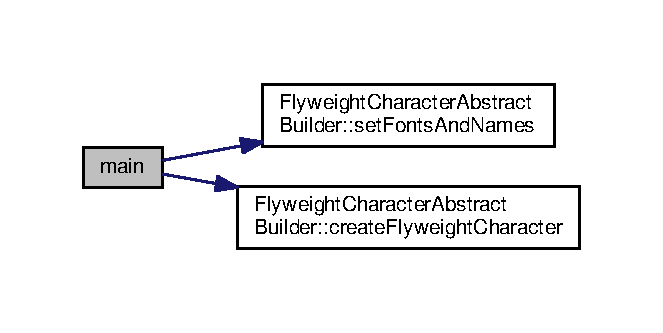
\includegraphics[width=318pt]{Flyweight_8cpp_a3c04138a5bfe5d72780bb7e82a18e627_cgraph}
\end{center}
\end{figure}



%--- End generated contents ---

% Index
\backmatter
\newpage
\phantomsection
\clearemptydoublepage
\addcontentsline{toc}{chapter}{Index}
\printindex

\end{document}
